\documentclass{beamer}

\usepackage[czech]{babel}				% Jazyk
\usepackage[a-2u]{pdfx}					% Kopírování z pdfka
\usepackage{tikz}						% Schémata automatů
\usepackage{csquotes}					% české uvozovky
\usepackage{enumerate}					% enumerate environment
\usepackage{indentfirst}
\usepackage{mathtools}
\usepackage{pifont}
\usepackage{xcolor}
\usepackage{enumitem,xcolor}
\usepackage{amsmath}
\usepackage[utf8]{inputenc}

\usepackage{listings}                   % Úryvky z kódu (C#)
\lstset{language=[Sharp]C, frame=lr}

% Assets
% Enumerate
%\setlist[enumerate]{topsep=0pt,itemsep=-1ex,partopsep=1ex,parsep=1ex,label=(\arabic*)}

\MakeOuterQuote{"}

% Colors
\definecolor{lightblue}{HTML}{009AD4}
\definecolor{darkgreen}{HTML}{0D7103}
\definecolor{lightgreen}{HTML}{68FF00}
\definecolor{darkred}{HTML}{AF0B0B}
\definecolor{lightred}{HTML}{FF5100}
\definecolor{orange}{HTML}{FFE000}
\definecolor{codeblue}{HTML}{FF0055}
\definecolor{codegreen}{rgb}{0,0.6,0}
\definecolor{codegray}{rgb}{0.5,0.5,0.5}
\definecolor{codebeige}{HTML}{D4A000}
\definecolor{backcolour}{rgb}{0.95,0.95,0.92}

\newcommand{\markred}[1]{\textcolor{lightred}{#1}}
\newcommand{\markgreen}[1]{\textcolor{lightgreen}{#1}}
\newcommand{\markorange}[1]{\textcolor{orange}{#1}}
\newcommand{\markblue}[1]{\textcolor{lightblue}{#1}}

% Inline images
\newcommand{\inlineimgscale}{1.1}

% X and check mark
\newcommand{\cmark}{\markgreen{\ding{51}}}
\newcommand{\xmark}{\markred{\ding{55}}}

% Redefinions
\renewcommand{\implies}{\Rightarrow}
\renewcommand{\impliedby}{\Leftarrow}

% Math
\newcommand{\R}{\mathbb{R}}
\newcommand{\C}{\mathbb{C}}
\newcommand{\N}{\mathbb{N}}
\newcommand{\Z}{\mathbb{Z}}
\newcommand{\Q}{\mathbb{Q}}

% Code
\lstdefinestyle{clang}{
    basicstyle=\small\ttfamily\color{white},
    language=C,
    keywordstyle=\color{codeblue},
    commentstyle=\color{codegreen},
    numberstyle=\tiny\color{codegray},
    stringstyle=\color{codebeige},
    breakatwhitespace=false,
    breaklines=true,
    captionpos=b,
    keepspaces=true,
    numbersep=5pt,
    showspaces=false,
    showstringspaces=false,
    showtabs=false,
    morekeywords={void,int,double,float,unsigned,if,else,\#include}
    tabsize=0.5
}
\lstset{escapeinside={(*}{*)},style=clang}

\newcommand{\hlcode}[1]{\colorbox{red}{#1}}

% Theme
\usetheme{Boadilla}
\setbeamertemplate{frame numbering}[fraction]
\usecolortheme[named=darkblue]{structure}
\setbeamertemplate{navigation symbols}{}

% Title page
\subtitle{Procvičování algoritmizace s polem}
\author{David Weber}
\date{\today}

\begin{document}

\defverbatim{\minmaxlookup}{\begin{verbatim}
int min = A[0]; int max = A[0];
int n = sizeof(A)/sizeof(int);

for (int i=0; i<n; i++){
    if (A[i] < min) min = A[i];
    if (A[i] > max) max = A[i];
}
\end{verbatim}}
\defverbatim{\elementlookup}{\begin{verbatim}
int element;
scanf("%d", &element);
int n = sizeof(A)/sizeof(int);
int index = -1;

for (int i=0; i<n; i++){
    if (A[i] == element){
        printf("%d\n", i);
        break;
    }
}
\end{verbatim}}
\defverbatim{\sumlookup}{\begin{verbatim}
int sum;
scanf("%d", &sum);
int n = sizeof(A)/sizeof(int);

for (int i=0; i<n; i++){
    for (int j=i+1; j<n; j++){
        if (A[i] + A[j]==sum)
            printf("i=%d, j=%d\n", i, j);
    }
}
\end{verbatim}}

    \begin{frame}[t]
        \titlepage
    \end{frame}

    \begin{frame}[t]{Opakování}
        \begin{itemize}
            \item datová struktura, která sdružuje dané prvky (čísla, textové řetězce, \dots) \textbf{stejného datového typu}.
            \item Velikost pole zůstává při běhu programu \textbf{neměnná}.
            \item K jednotlivým prvkům přistupujeme pomocí tzv. \emph{indexu} (celé číslo od $0$ do $n-1$.)
        \end{itemize}
        \begin{figure}
            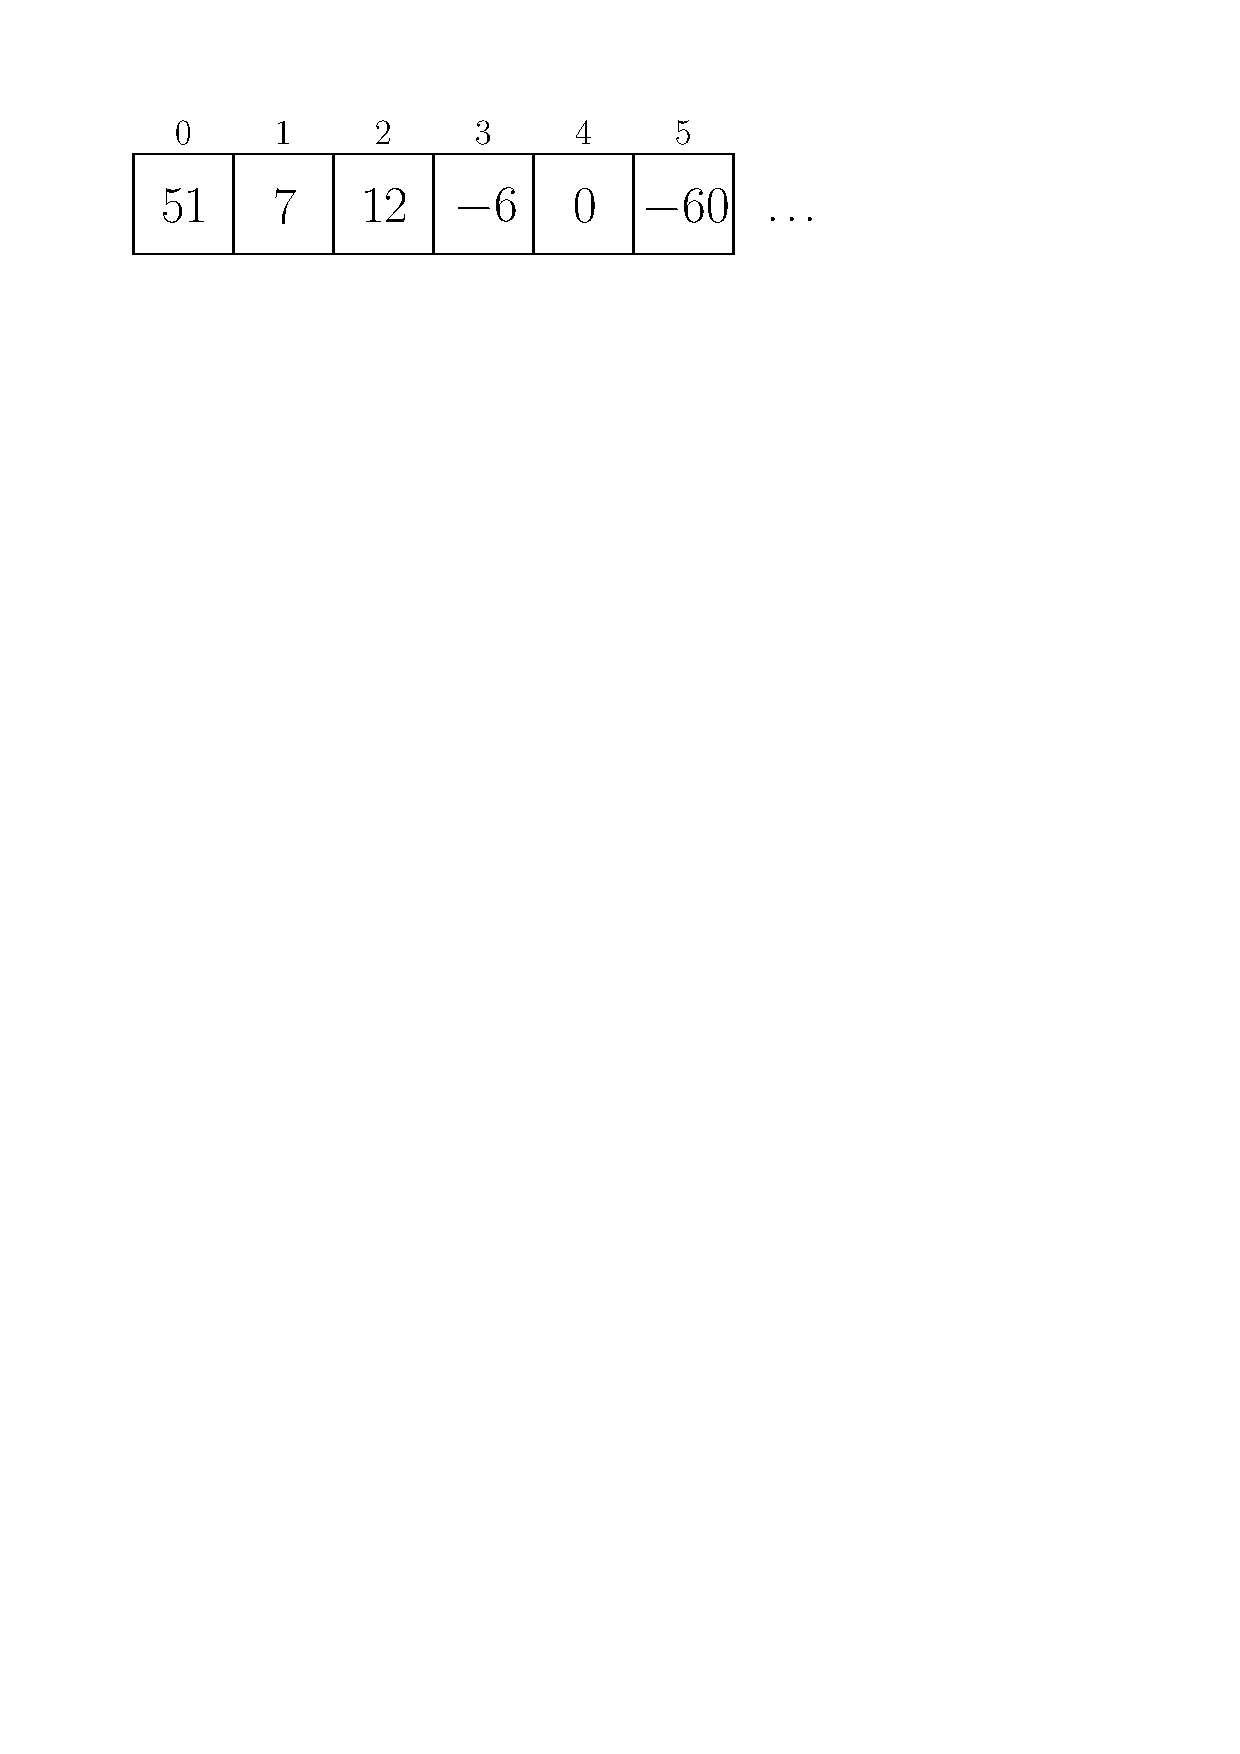
\includegraphics[scale=.8]{images/pole.pdf}
        \end{figure}
    \end{frame}

    \begin{frame}{Na rozehřátí}
        \only<2->{\begin{itemize}
            \item \textit{\textbf{Úloha:}} Napište algoritmus, který pro libovolné pole obsahující prvky typu \emph{integer} nalezne \textbf{minimum} a \textbf{maximum} a vypíše jej.
            \only<3->{\item \textit{\textbf{Úloha:}} Napište algoritmus, který pro \textbf{uživatelem zadané číslo} vyhledá a vypíše index prvního jeho výskytu v poli. Pokud se zadaný prvek v poli nenachází, vypíše $-1$.}
        \end{itemize}}
    \end{frame}

    \begin{frame}{Vzorové řešení první úlohy}
        \minmaxlookup
    \end{frame}

    \begin{frame}{Vzorové řešení druhé úlohy}
        \elementlookup
    \end{frame}

    \begin{frame}{Nyní těžší úlohy\dots}
        \only<2->{\begin{itemize}
            \item \textit{\textbf{Úloha:}} Napište algoritmus, který pro uživatelem zadané číslo $S$ vypíše \textbf{všechny} dvojice indexů $i, j$ v poli $A$, takové, že
            \[A[i]+A[j]=S.\]
            (Tj. příslušná dvojice prvků je rovna zadanému součtu.)
            \only<3->{\item Zaveďte do svého algoritmu počítadlo kroků, tak, aby se zvýšilo při každém provedeném porovnání a na konci jej vypište.}
        \end{itemize}}
    \end{frame}

    \begin{frame}
        \sumlookup
    \end{frame}

    \begin{frame}{Optimalizace}
        \only<2->{\begin{itemize}
            \item Při návrhu algoritmu se vždy snažíme ideálně o co nejoptimálnější řešení.
            \only<3->{\item Naším cílem tak je dosáhnout správného výsledku pomocí co nejméně kroků $\implies$ šetříme čas a algoritmus lze použít i na větší vstupy.}
        \end{itemize}}
        \only<4->{Byl by Vámi navržený algoritmus optimální, pokud bychom pracovali se \textbf{setříděným polem}? Můžeme této vlastnosti nějak využít?\\}
    \end{frame}

\end{document}